\frame
{
\frametitle{\citetitle{MarcoNuno_CongArbIng_2005_09_00}}
\begin{columns}
    \column {0.5\textwidth}
\begin{itemize}    
\item Existe una variedad de técnicas de interpolación que pueden
ser utilizado para funciones tales como ampliar o reducir la
tamaño de una imagen. 
\item Los tres algoritmos muy utilizados son: vecino más cercano,
bilineal y bicúbica.
\end{itemize}
    \column {0.5\textwidth} 
    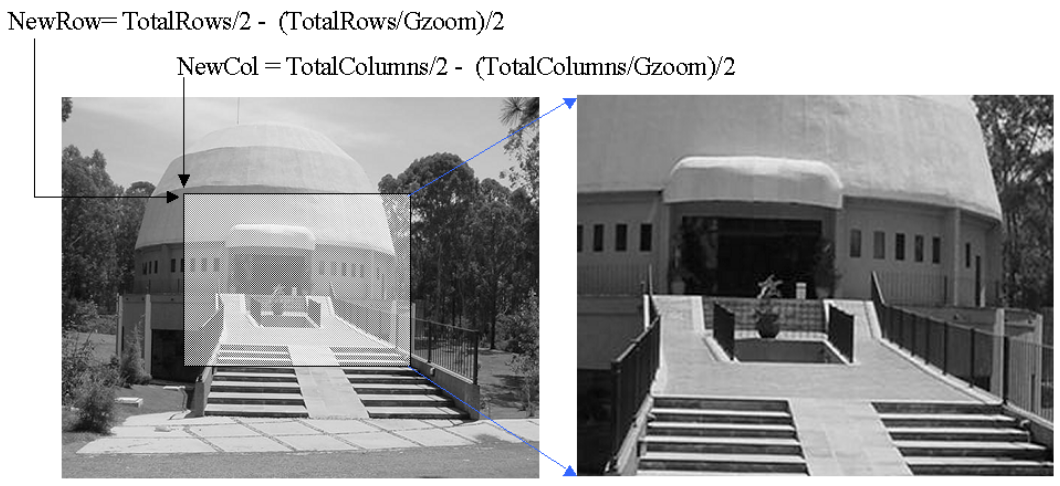
\includegraphics[width=0.9\textwidth]{Figs/BicubicInterpolation02}
\end{columns}     

\footnotetext[1]{\fullcite{MarcoNuno_CongArbIng_2005_09_00}}
}

\frame{
\frametitle{Arquitectura Propuesta}
\begin{columns}
    \column {0.5\textwidth}
    \begin{itemize}    
\item Un conjunto de procesadores de zoom (ZP) realizan el
operaciones entre los píxeles de la imagen de entrada y los coeficientes de interpolación, generando como salida el pixel de la  imagen resultante.
\item La interpolación bicúbica requiere una vecindad de 16
píxeles, 16 operaciones de punto flotante y hay similitud
con procesado de ventana.
\item En la implementación actual, se utiliza un Pipeline de $N$ etapas para acelerar el procesamiento de la interpolación.
\end{itemize}

    
    \column {0.5\textwidth} 
    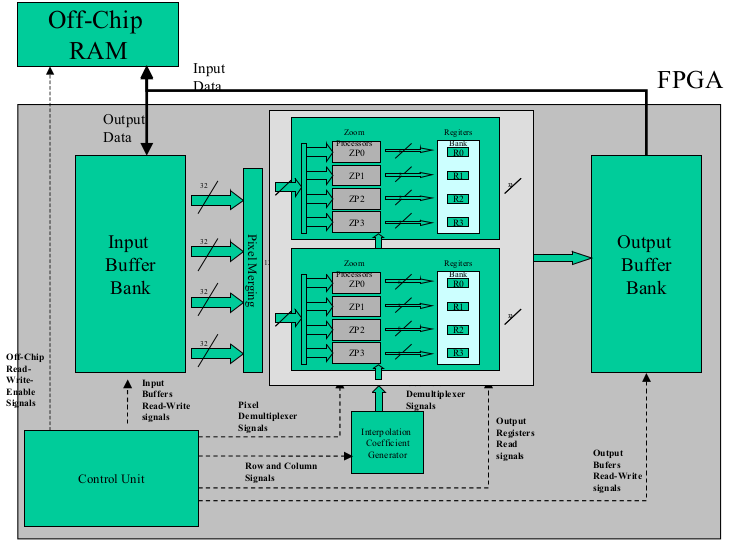
\includegraphics[width=0.9\textwidth]{Figs/BicubicInterpolation01}
\end{columns}     
}

\frame{
\frametitle{Implementación y Resultados}
\begin{columns}
    \column {0.5\textwidth}
    \begin{itemize} 
\item Se comparó el trabajo propuesto con otros trabajos existentes en la literatura
\item El trabajo propuesto procesa una imágen en 3.5 ms, mientras que el más cercano requería de 11 ms.
\item La implementación de la interpolación del lado de la PC requirió de 50ms para completarse.
\end{itemize}
    \column {0.5\textwidth} 
    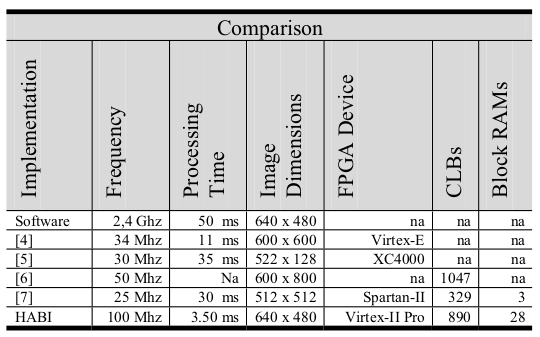
\includegraphics[width=0.9\textwidth]{Figs/BicubicInterpolation03}
\end{columns}     
}
